\documentclass[xcolor=pdftex,x11names,table,hyperref]{beamer}

\usepackage{verbatim}
\usepackage{setspace}
\usepackage{url}
\usepackage{xcolor} % See documentation PDF at http://www.ctan.org/pkg/xcolor
\definecolor{darkgreen}{rgb}{0,0.3,0}
\definecolor{darkblue}{rgb}{.05,.05,.30}
\definecolor{lightgrey}{rgb}{0.65,0.65,0.65}
\usepackage{tikzsymbols}


\setbeamertemplate{section in toc}[sections numbered]
\setbeamertemplate{subsection in toc}[subsections numbered]
\setbeamertemplate{subsubsection in toc}[subsubsections numbered]
\usetheme{Singapore}
\setbeamertemplate{navigation symbols}{}
\setbeamertemplate{footline}{%
\vspace{0.0em}%
\hspace{0.5em}%
{\color[rgb]{.1,.1,.1} \insertframenumber{}~/~\inserttotalframenumber}
}

\newcommand{\code}[1]{{\color{darkgreen}\texttt{#1}}}
\newcommand{\detail}[1]{{\color{lightgrey}\small{}#1}}
\newcommand{\teeny}[1]{\scalebox{0.09}{#1}}
\newcommand{\tablecolors}{\rowcolors{2}{blue!12}{white}} % Cool table colors
\newcommand{\conv}{convolutional}
\newcommand{\Conv}{Convolutional}


\begin{document}

\title{\Conv{} Neural Nets \\[1.5em]
 %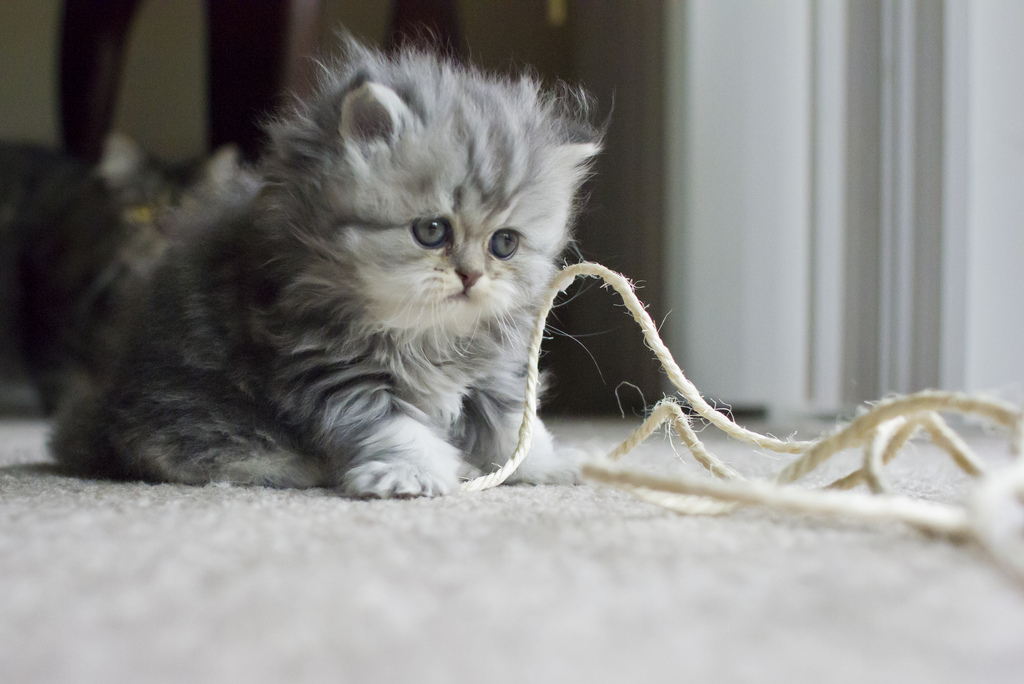
\includegraphics[width=0.5\textwidth]{images/kitten_string_flickr_albaraa.jpg} \\[-1.0em]
 \small{and Character-based Language Models} \\[1.0em]
 %LT1 \\[1.0em]
 }
\author{\href{http://jon.dehdari.org}{Jon Dehdari}}
\frame{\titlepage}

%\begin{frame}{Good Morning!}
%	\begin{center}
%	%\includegraphics[width=0.8\textwidth]{images/.jpg}
%	\end{center}
%\end{frame}

\begin{frame}{Too Connected!}
\begin{itemize}
	\item All the neural networks that we've seen so far are \emph{fully connected} between each layer
	\item That is, every node in a layer is connected to every node in the next layer
	\begin{center}
	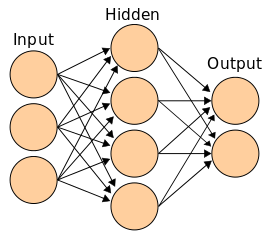
\includegraphics[width=0.3\textwidth]{images/wp_artificial_neural_network.png}
	\end{center}
	\pause
	\item This is fine for small inputs, but not for large inputs
\end{itemize}
\end{frame}

% fully connected ("It's all connected!") vs CNNs and pooling (max, avg, ): use low-level features to form high-level generalizations

\begin{frame}{\Conv{} Neural Network (CNN)}
\begin{itemize}
	\item Convolutional layers localize connections to a small window of input
	\begin{center}
	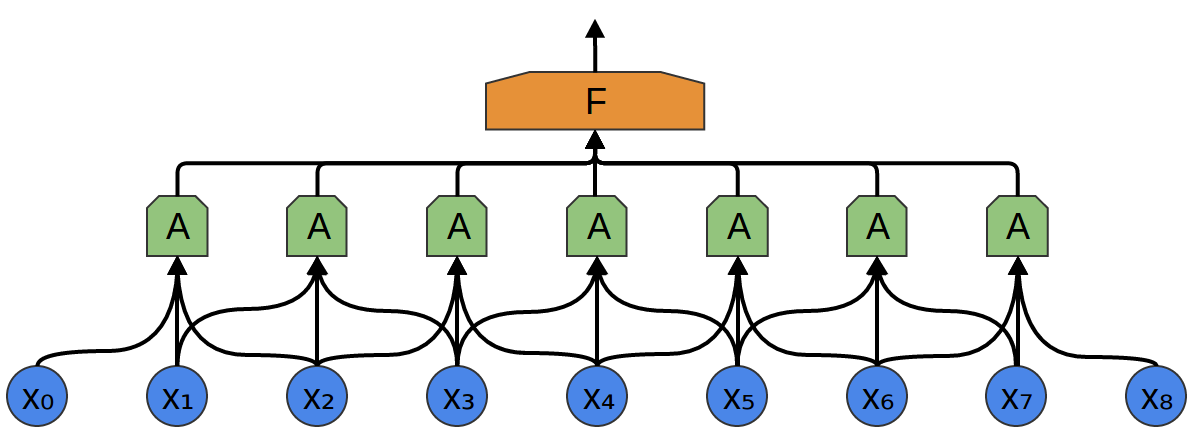
\includegraphics[width=0.7\textwidth]{images/colah_Conv-9-Conv3.png}
	\end{center}
	\pause
	\item Here the input node $x_3$ connects to the second, third, and fourth nodes at the next layer
\end{itemize}
\teeny{Image courtesy of \href{https://colah.github.io/posts/2014-07-Conv-Nets-Modular}{Colah's awesome blog}}
\end{frame}

% Assumes spacial (or maybe temporal) relationship of input

\begin{frame}{Convolutions}
\begin{itemize}
	\item A convolution in this context is just the dot product of a window of input and its weight matrix:
	\begin{center}
	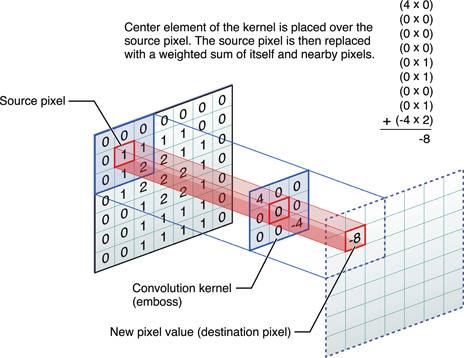
\includegraphics[height=0.47\textheight]{images/apple_kernel_convolution.jpg}
	\end{center}
	\pause
	\item It's also sometimes called a filter or kernel, because CNNs were originally popular with image processing
	\pause
	\item It's common to use the same weight matrix at all positions \detail{(parameter sharing)}, because a cat is a cat regardless of where in the image it is!
\end{itemize}
\teeny{Image courtesy of \href{https://developer.apple.com/library/ios/documentation/Performance/Conceptual/vImage/ConvolutionOperations/ConvolutionOperations.html}{Apple}}
\end{frame}

% windows, stride

\begin{frame}{Pool Party!}
\begin{itemize}
	\item \textbf{Pooling} takes the maximum value (``max pooling'') or arithmetic mean (``average pooling'') of a small block of nodes
	\begin{center}
	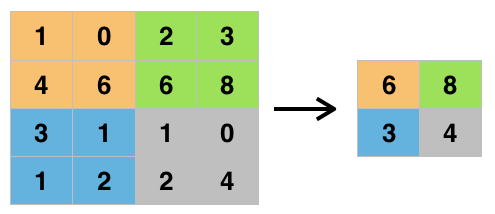
\includegraphics[height=0.4\textheight]{images/wp_max_pooling.png}
	\end{center}
	\pause
	\item We can view pooling as ``summarizing'' a low-level area of input
	\item They allow small variations of input \detail{\small{(translation invariance)}}, and preventing overfitting
	\pause
	\item Pooling layers are usually on top of a \conv{} layer
\end{itemize}
\teeny{Image courtesy of \href{https://commons.wikimedia.org/wiki/File:Max_pooling.png}{Wikipedia}}
\end{frame}

\begin{frame}{Combining \Conv{} Layers and Pooling}
\begin{itemize}
	\item We can combine a \conv{} layer and max pooling:
	\begin{center}
	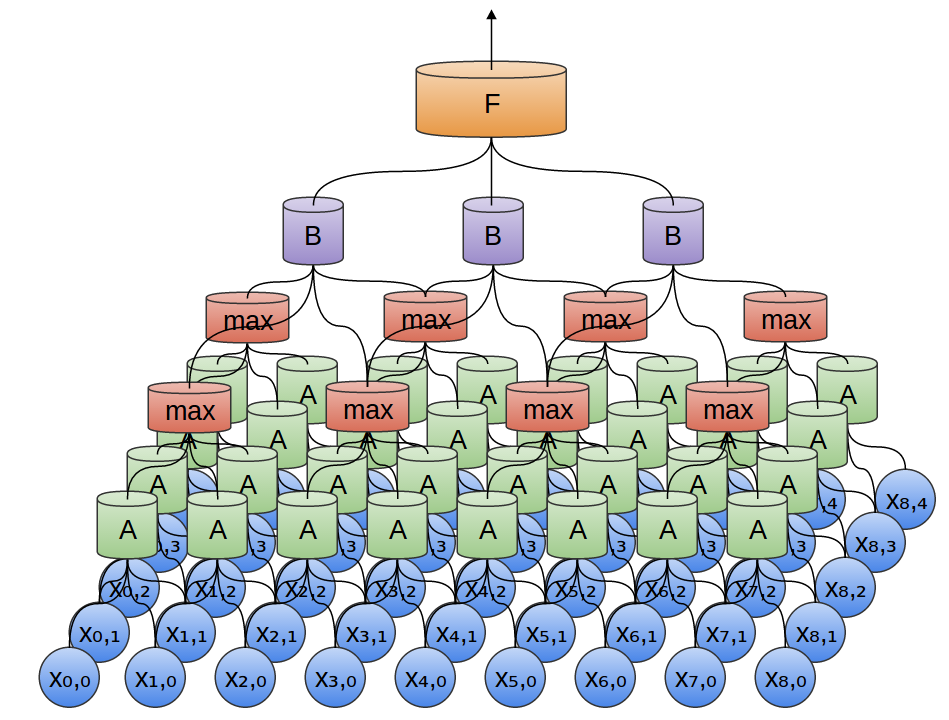
\includegraphics[height=0.63\textheight]{images/colah_Conv2-9x5-Conv2Max2Conv2.png}
	\end{center}
\item The 2-dim.\ input is blue, then a \conv{} layer (green), then a max pooling layer (red), then another conv.\ layer (purple), and finally a fully-connected layer is orange
\end{itemize}
\teeny{Image courtesy of \href{https://colah.github.io/posts/2014-07-Conv-Nets-Modular}{Colah's awesome blog}}
\end{frame}

% show edge-detection visual example

% application to CV

\begin{frame}{Face Detection Example}
%\begin{itemize}
	%\item 
	%\item 
	\begin{center}
	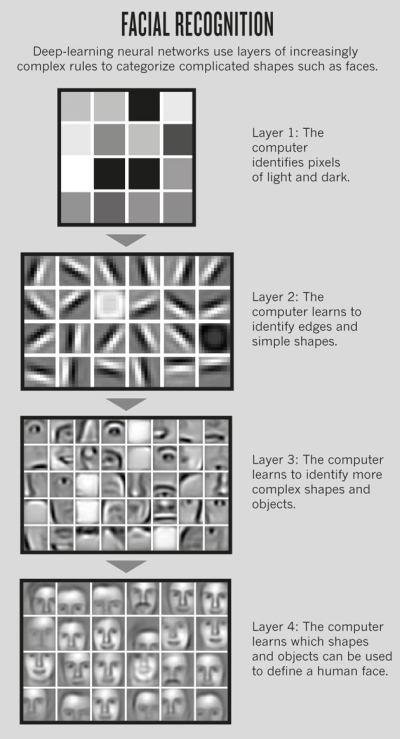
\includegraphics[height=0.90\textheight]{images/deep_cnn_face.jpg}
	\end{center}
%\end{itemize}
\end{frame}

% application to char-lm's, citing harvard group's paper ( http://arxiv.org/abs/1508.06615 )
\begin{frame}{Character-based Neural Language Models}
\begin{itemize}
	\item \href{http://arxiv.org/abs/1508.06615}{Kim et al. (2016)} made a nice character-based language model by combining \conv{} layers, LSTMs, and highway networks (like LSTMs for deep networks): \\
	\begin{center}
	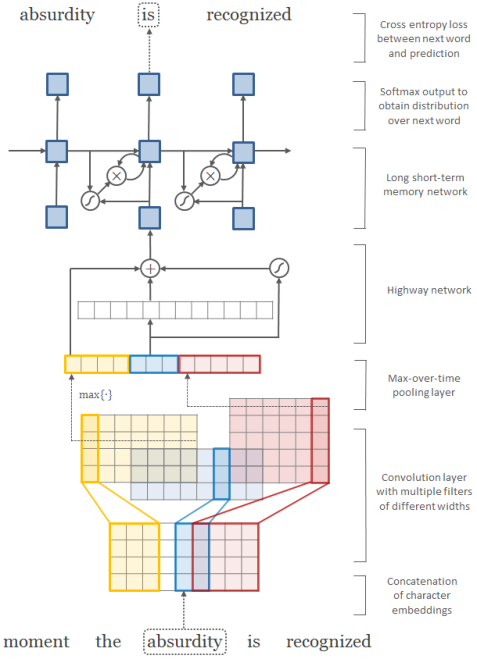
\includegraphics[height=0.73\textheight]{images/kim-etal2016_fig1.pdf}
	\end{center}
\end{itemize}
\end{frame}

\begin{frame}{Character-based Neural Language Models (cont'd)}
	\begin{center}
	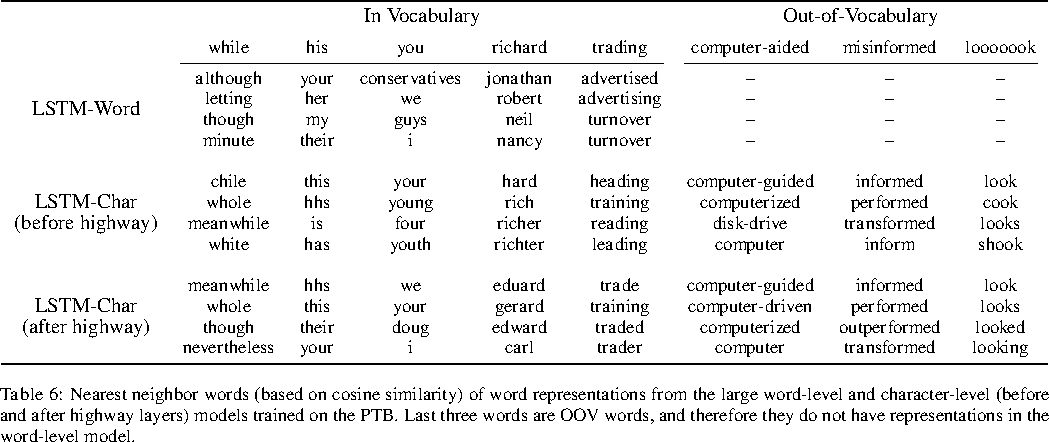
\includegraphics[width=1.02\textwidth]{images/kim-etal2016_table6.pdf}
	\end{center}
\end{frame}


% ?? recursive NNs


\begin{frame}{Further Reading}
\textbf{Overviews}:
\begin{tiny}
\begin{itemize}
	\item \url{http://u.cs.biu.ac.il/~yogo/nnlp.pdf} (\S{} 9)
	\item \url{https://colah.github.io/posts/2014-07-Conv-Nets-Modular}
	\item \url{https://colah.github.io/posts/2014-07-Understanding-Convolutions}
	\item \url{https://colah.github.io/posts/2014-12-Groups-Convolution}
	\item \url{http://neuralnetworksanddeeplearning.com/chap6.html}
	\item \url{https://en.wikipedia.org/wiki/Convolutional_neural_network}
	\item \url{http://white.stanford.edu/teach/index.php/An_Introduction_to_Convolutional_Neural_Networks}
	\item \url{http://deeplearning.net/tutorial/lenet.html}
	\item \url{https://cs231n.github.io/convolutional-networks}
	\item \url{http://cs224d.stanford.edu/lectures/CS224d-Lecture13.pdf}
\end{itemize}
\end{tiny}
\textbf{Original Papers}:
\begin{tiny}
\begin{itemize}
	\item LeCun, Yann, \& Bengio, Yoshua. 1995. \href{http://www.iro.umontreal.ca/~lisa/pointeurs/handbook-convo.pdf}{\Conv{} networks for images, speech, and time series}. \textit{The handbook of brain theory and neural networks}, 3361.10.
	\item Kim, Yoon, Yacine Jernite, David Sontag, Alexander M. Rush. 2016. \href{http://arxiv.org/abs/1508.06615}{Character-Aware Neural Language Models}.  In \textit{Proceedings of AAAI-2016}. Phoenix, AZ, USA. \href{http://arxiv.org/abs/1508.06615}{arXiv:1508.06615}. \href{https://github.com/yoonkim/lstm-char-cnn}{Software Link}.
\end{itemize}
\end{tiny}
\end{frame}





% \begin{frame}{}
% \begin{itemize}
% 	\item 
% 	\item 
% 	\item 
% \end{itemize}
% \end{frame}


\end{document}
